%%%%%%%%%%%%%%%%%%%%%%%%%%%%%%%%%%%%%%%%%%%%%%%%%%%%%%%%%%%%%%%%%%%%%%%%%%%%%%%%
%2345678901234567890123456789012345678901234567890123456789012345678901234567890
%        1         2         3         4         5         6         7         8

\documentclass[letterpaper, 10 pt, conference]{ieeeconf}  % Comment this line out if you need a4paper

%\documentclass[a4paper, 10pt, conference]{ieeeconf}      % Use this line for a4 paper

\IEEEoverridecommandlockouts                              % This command is only needed if 
                                                          % you want to use the \thanks command

\overrideIEEEmargins                                      % Needed to meet printer requirements.

% See the \addtolength command later in the file to balance the column lengths
% on the last page of the document

% The following packages can be found on http:\\www.ctan.org
%\usepackage{graphics} % for pdf, bitmapped graphics files
%\usepackage{epsfig} % for postscript graphics files
%\usepackage{mathptmx} % assumes new font selection scheme installed
%\usepackage{times} % assumes new font selection scheme installed
%\usepackage{amsmath} % assumes amsmath package installed
%\usepackage{amssymb}  % assumes amsmath package installed
\usepackage{graphicx}
\usepackage[export]{adjustbox}
\graphicspath{ {images/} }


\title{\LARGE \bf
Duckiebot with Blind Navigation
}


\author{YuHsin Wu$^{1}$ and Michael Su$^{2}$% <-this % stops a space
\thanks{*This work was supported by the Robotics Master Program in National Chiao Tung University, Taiwan}% <-this % stops a space
\thanks{$^{1}$YuHsin Wu is with National Chiao Tung University, Taiwan.
        {\tt\small whish713.eed04@g2.nctu.edu.tw}}%
\thanks{$^{2}$Michael Su,
        {\tt\small b.d.researcher@ieee.org}}%
}


\begin{document}



\maketitle
\thispagestyle{empty}
\pagestyle{empty}


\section{INTRODUCTION \& MOTIVATION}

Inspired by Wang~\cite{wang2017enabling}, we want to apply duckiebot on blind navigation. The original duckiebot~\cite{paull2017duckietown} runs according to the yellow and white lines on the road and it can run well in the fixed map. Now we hope that our duckiebot can run on the real world, so that our duckiebot can lead blind people to the destination safely. In our duckiebot, we will equip it with a range sensor Asus Xtion, and replace the original line detector and lane filter with a depth line detector and corresponding lane filter to enable our duckiebot to find where the road is. We hope that the blind people's action won't be limited anymore.

\section{SYSTEM ARCHITECTURE \& EQUIPMENTS}



\subsection{SYSTEM ARCHITECTURE}
\begin{figure}[h!] % h means put this image here
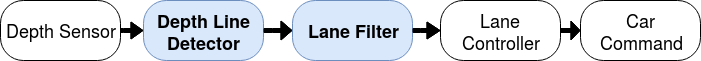
\includegraphics[width=1.0\columnwidth]{system_flowchart.png}
\centering
\caption{system flowchart}
\end{figure}

Generally, the architecture is similar to the original duckietown lanefollowing. Different from the original version, our depth line detector will replace the original line detector and groud projection. The input of depthl 1ine detector is pointcloud instead of rgb image. The new detector will detect two walls on both sides of the road, and these two walls are trasformed into line segments which represent the direction of road. The output is the line segments of walls which are the same as original lanefollowing. 

In original lane filter, the lane width is fixed. To apply depth line detector on the real world, we hope our car is able to run on the road of non-fixed width. To enable our duckiebot to go straight in the center of roads of different width, we revise the lane filter to a dynamic-lane-width lane filter. Except the depth line detector and the dynamic-lane-width lane filter, our architecture is the same as the original duckietown.


\subsection{EQUIPMENTS} 

Our duckiebot is equipped with a range sensor Asus Xtion, whice can observe the environment ranging from 0.5 to 10 meters. Furthermore, A rod~\cite{wei2014guide} and a set of strong-torque motors are used to lead the visually impaired.

\begin{figure}[t] % t means put this image at the top 
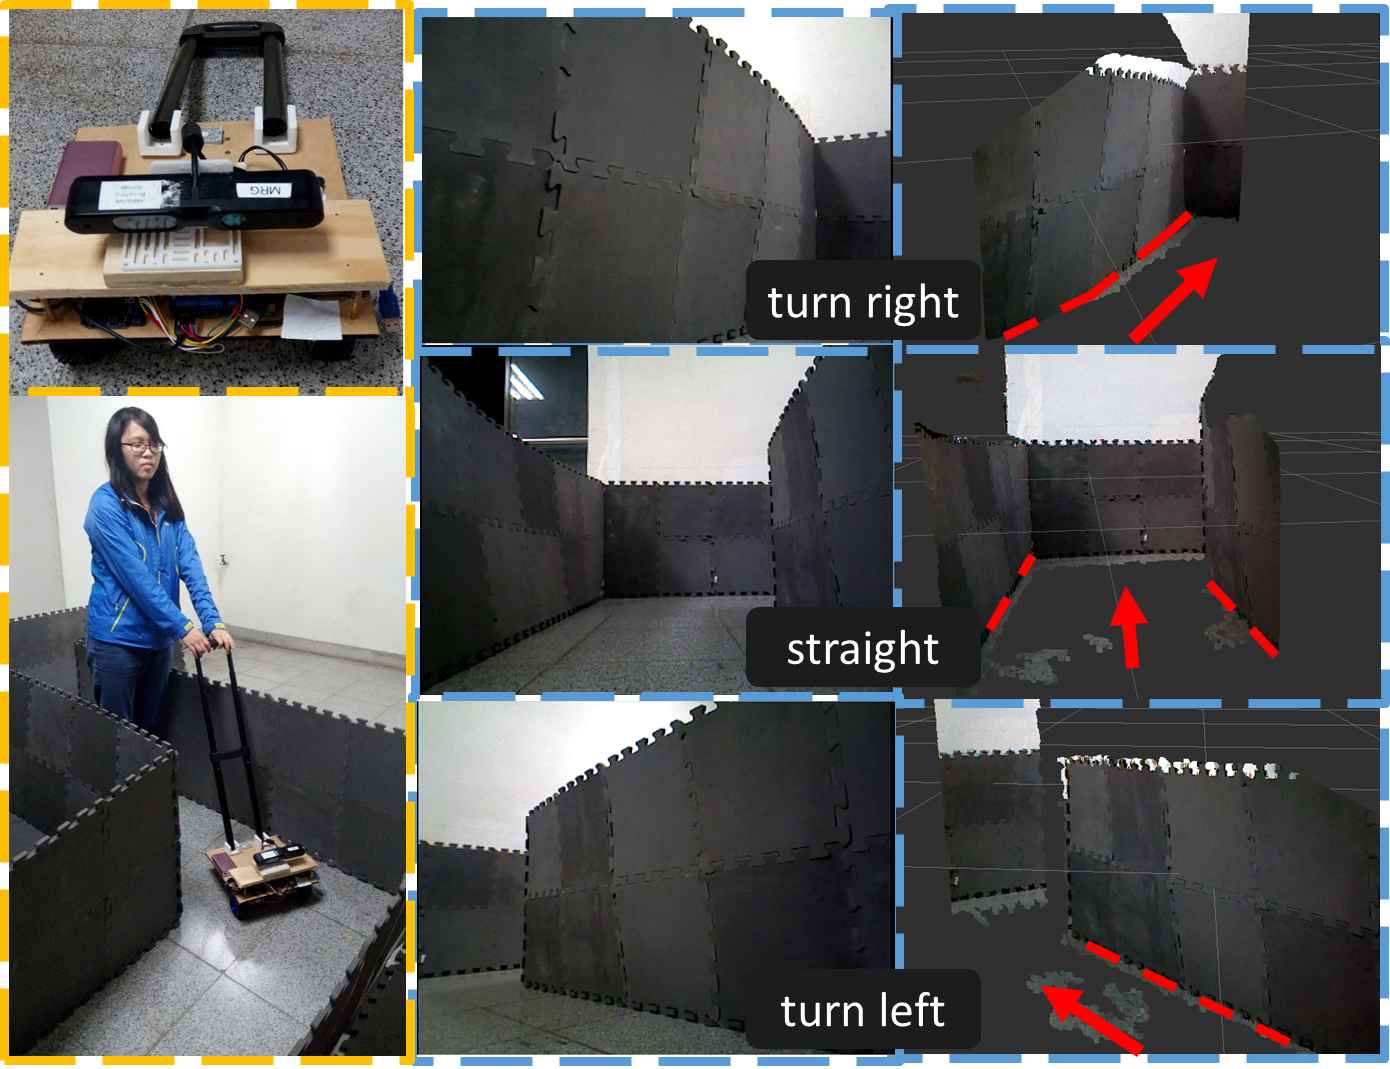
\includegraphics[width=1.0\columnwidth]{teaser.png}
\centering
\caption{The upper left is the duckiebot, the bottom left is user using the duckiebot, the right part is the sensor input in different situation.}
\end{figure}

\section{SPECIFIC AIMS}

\begin{figure}[h!] % h means put this image here
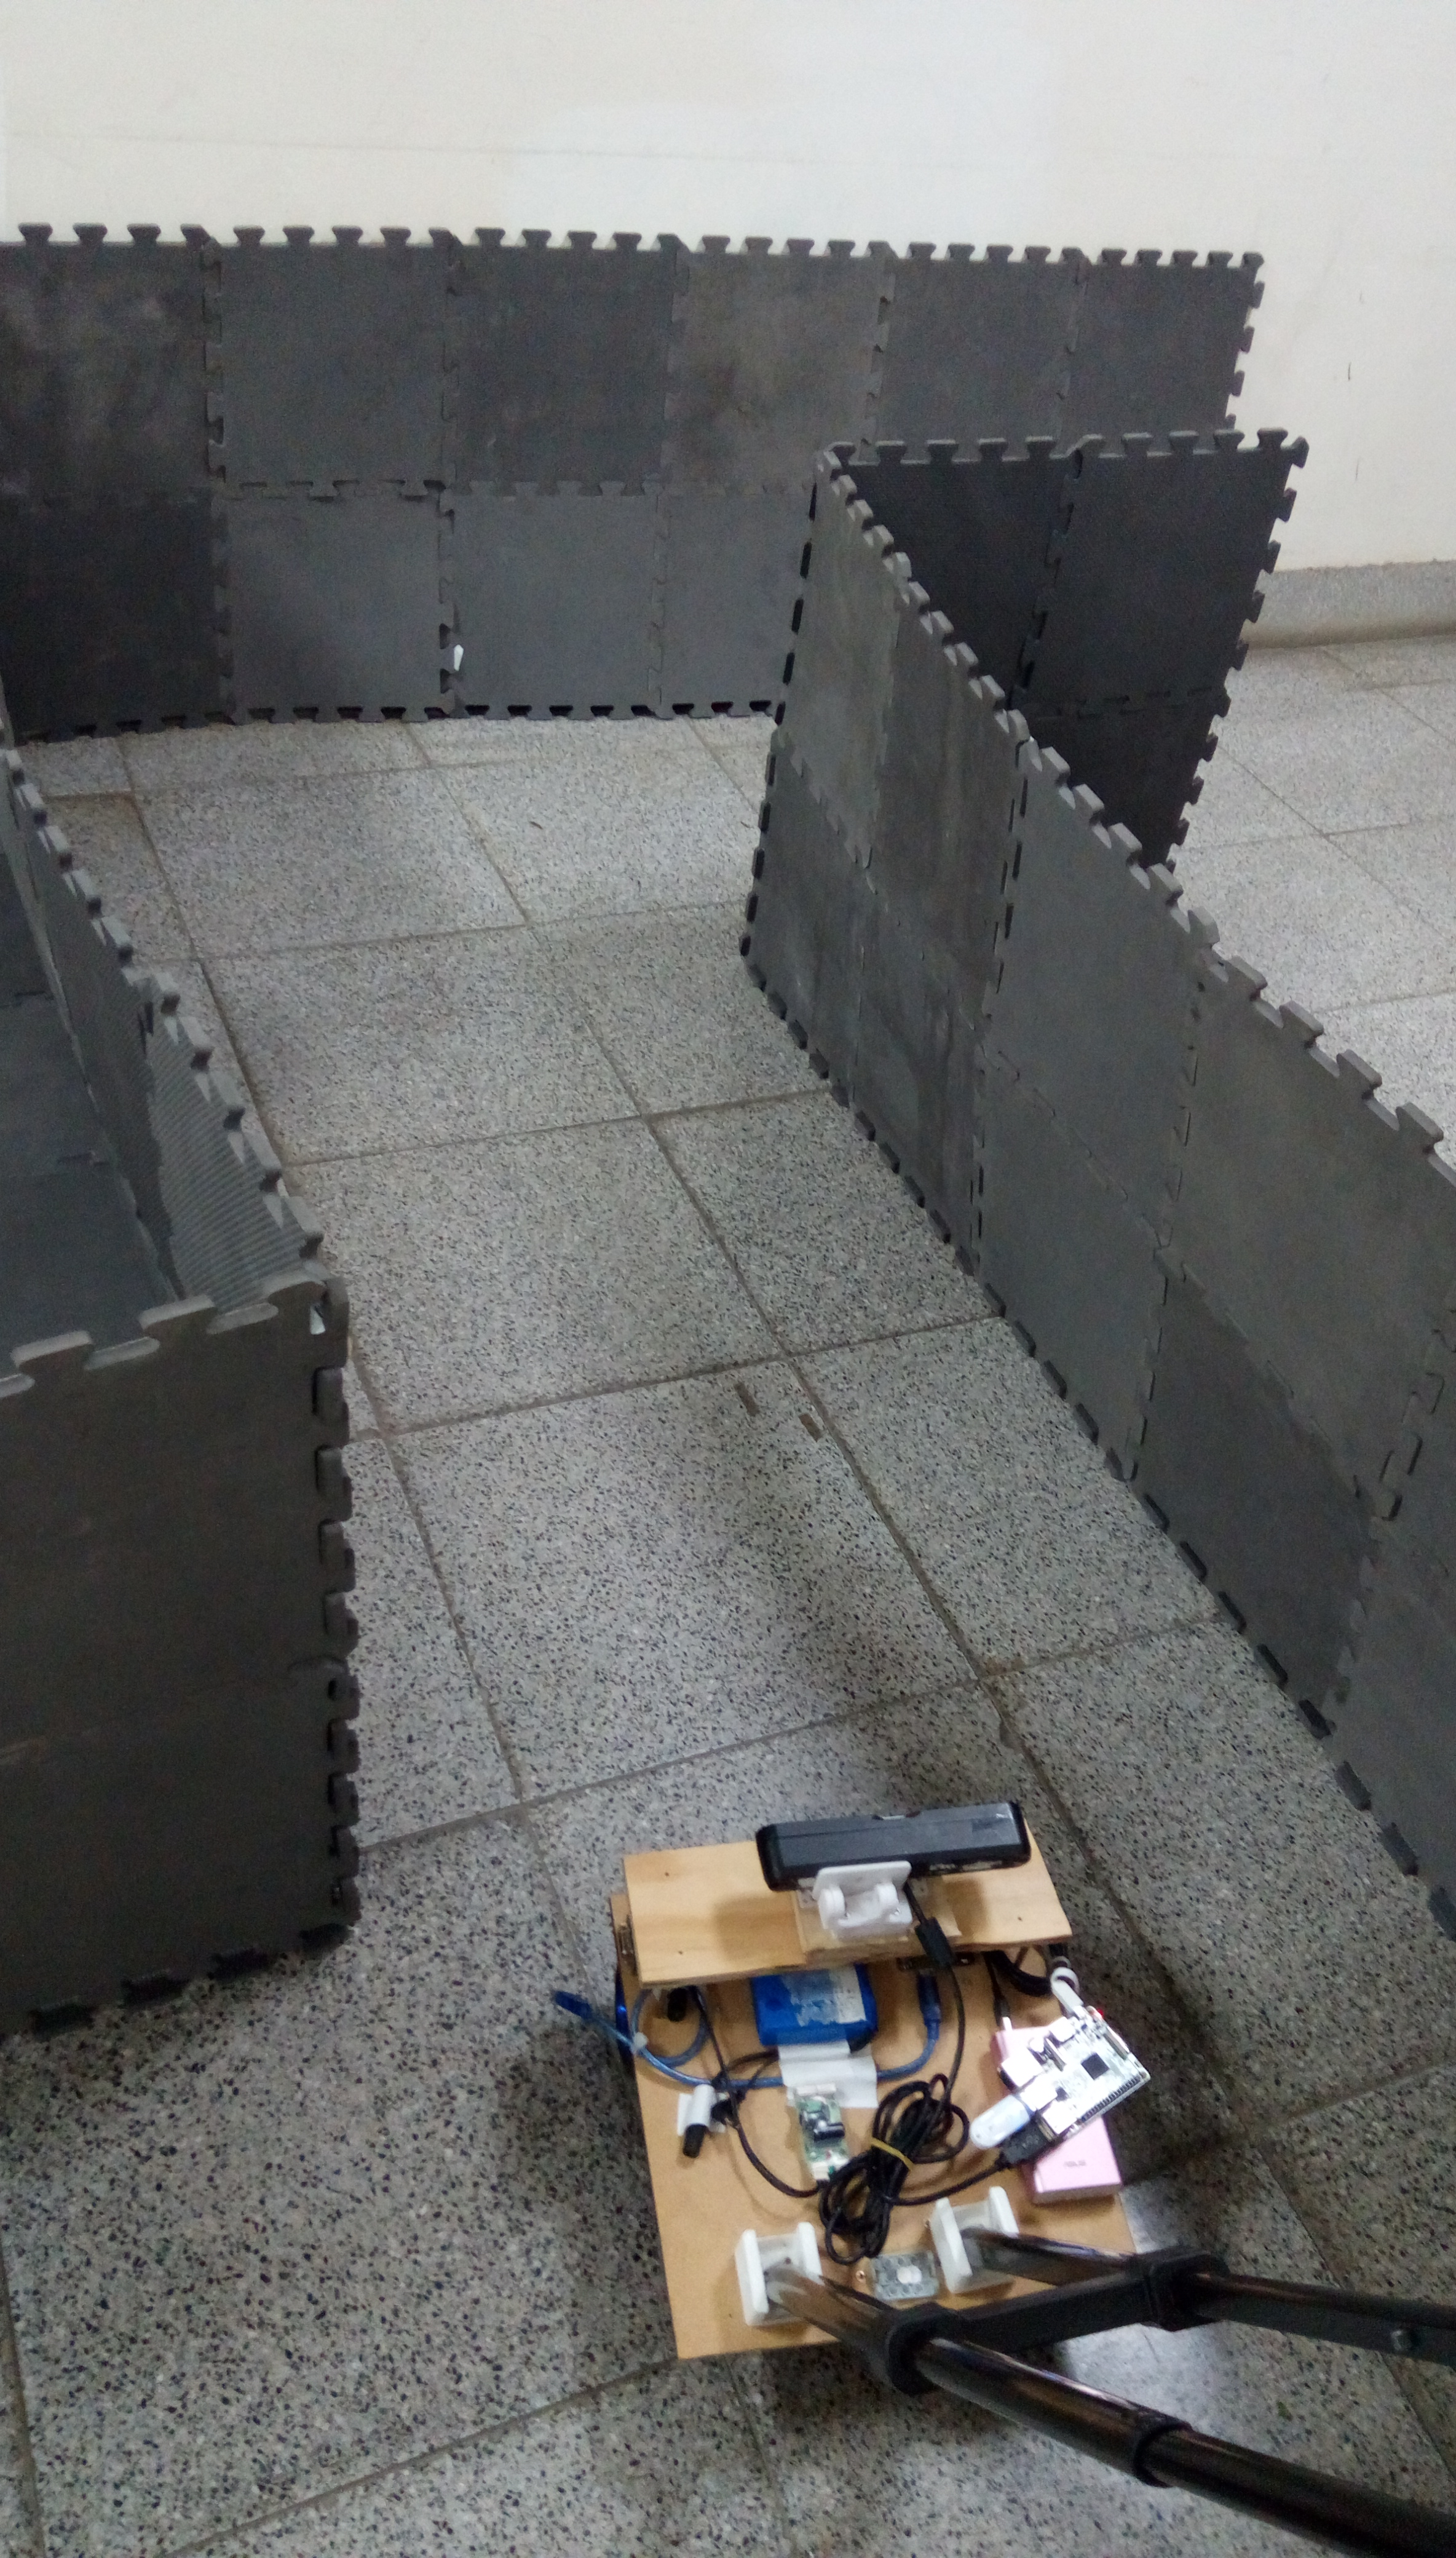
\includegraphics[width=0.8\columnwidth]{map.jpg}
\centering
\caption{The experiment environment is a map in shape of a lightning bolt, the duckiebot needs to turn left and right in order to get to the end. 
}
\end{figure}

\begin{itemize}

\item Specific Aim 1.

Dukiebot can go through a map which has fixed lane width.
\item Specific Aim 2.

Dukiebot can go through a map which has dynamic lane width.
\end{itemize}

\section{APPROACH}


\begin{figure}[ht] % h means put this image here
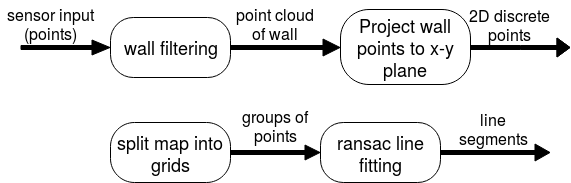
\includegraphics[width=1.0\columnwidth]{approach1.png}
\centering
\caption{approach flowchart}
\end{figure}

\begin{itemize}

\item Wall filtering.\\ 
Supposing that the sensor is horizontal to the ground, the normal of the wall is horizontal to the ground, and the normal of the road is vertical to the ground. Using this property, we can easily classify points as wall or ground.

\item Project wall points.\\ 
With these points of wall, we can't still determine which way to go, so we need to project the wall to x-y plane, then form 2D discrete points. These projected points seem like two lines and imply the trend of the road. 

\item Split map.\\ 
To describe the road, we split the map into lots of grids. There are many points in each grid, and they can be seen as a road segment.

\item Random sample consensus (RANSAC) line fitting.\\ 
RANSAC~\cite{fischler1981random, Rusu_ICRA2011_PCL} is an iterative method to estimate parameters of a mathematical model from a set of observed points. We will use RANSAC to fit these discrete points in every grid as a line segment and produce the line segment list.

\end{itemize}

\begin{figure}[h!] % h means put this image here
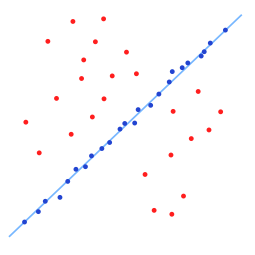
\includegraphics[width=0.5\columnwidth]{RANSAC.png}
\centering
\caption{Fitted line with RANSAC; outliers have no influence on the result.}
\end{figure}




\section{SCHEDULE AND TEAM COLLABORATION}
\begin{figure}[h!] % h means put this image here
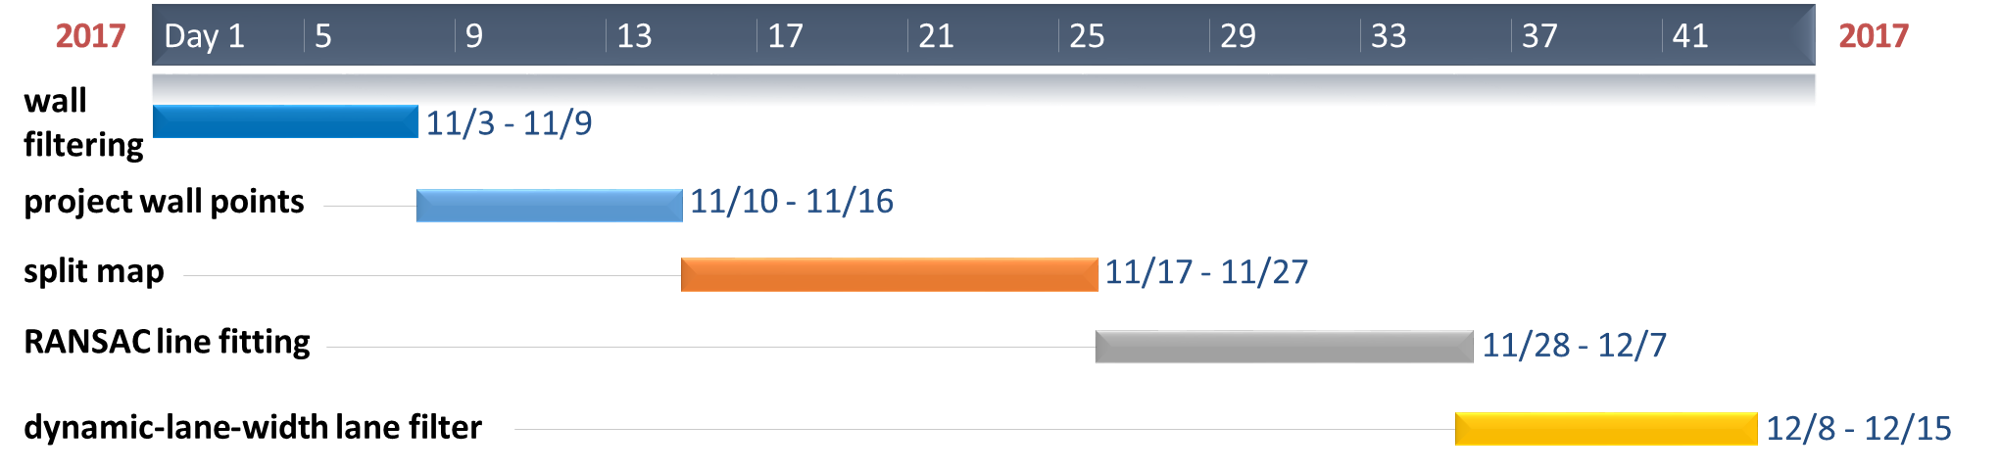
\includegraphics[width=1.0\columnwidth]{schedule.png}
\centering
\caption{schedule 
}
\end{figure}


\addtolength{\textheight}{-12cm}   % This command serves to balance the column lengths
                                  % on the last page of the document manually. It shortens
                                  % the textheight of the last page by a suitable amount.
                                  % This command does not take effect until the next page
                                  % so it should come on the page before the last. Make
                                  % sure that you do not shorten the textheight too much.

\bibliographystyle{IEEEtran}
\bibliography{egbib}

\end{document}
